\documentclass{article}

\usepackage{url}
\usepackage{graphicx}
\usepackage[width=4.5in,height=7.2in]{geometry}

\title{Drawing Trees and Animating Tree Changes}

\author{Sandro Badame, Peter Boothe\footnote{Corresponding author}\\
 Manhattan College\\
\url{{sbadame.student,peter.boothe}@manhattan.edu}}

\newcommand{\newword}[1]{\textit{#1}\index{#1}}
\newcommand{\java}[1]{\texttt{#1}\index{#1}}

\begin{document}
\maketitle

\begin{abstract} Dynamic trees appear in many areas of computer science,
including, but not limited to, Lisp code, data structures, tree automata, and
computer algorithms.  It would be useful to be able to easily draw trees and
animate them changing over time.  We articulate a design for tree
visualization and animation that is more general than previous methodologies.
Our design is enabled by the observation that, for trees which are small enough
to be displayed on a screen, computers are now fast enough to eliminate many
concerns about efficiency.  This observation allows us to make a library which
emphasizes simplicity of use over efficiency of execution.  We show how to use  our
library using several visualizations.\end{abstract}

\section{Introduction}
Trees, and especially trees which change over time, are fundamental objects in
computer science.  They occur in many disparate contexts, and while the uses of
these trees may be different, there exist commonalities which we exploit to
build a tree visualization system which might be useful in many different
contexts.  We will articulate the design principles of a highly usable
tree visualization system, present one such system that we have built in Java
and made freely available, and then show our system's utility with
several sample visualizations.

There are multiple reasons to visualize a system, and different reasons have
different requirements.  A visualization designed for experts may be very
useful for that target group, but leave neophytes confused.  Therefore, before
we discuss the particulars of our visualization, we must explain our reasons
for wanting such a system in the first place, as well as identify the expected
audience.  We want to visualize dynamic trees for demonstration, education, and
beauty, and we would like our system to be of benefit to computer
science undergraduates.

\subsection{Visualization for Demonstration}

One reason for visualization is for demonstration.  Trees and other systems
are visualized in an effort to show how these systems work.  Because this is
one of our goals, we will restrict ourselves to trees which are small enough to
be drawn in their entirety on a single computer screen.  Whenever we visualize a tree, our display system will show the entire tree, and it will be part of the job of our library to make the best use of the available screen real estate.

\subsection{Visualization for Education}
\label{educ}

Computing and math educators have a long history of building visualization
systems for demonstration.  The intuition was that if students could view these
systems in action, then the students would understand these systems.
Unfortunately for those goals, Hundhausen, Douglas, and Stasko found that, in practice, almost all
visualizations are useless\cite{hds}.  A good visualization seems intuitively helpful, but
it turns out that if a student does not understand the system being visualized, they will not understand the visualization either.  The one bright spot in this was in interactivity and construction.  The activity that improved student understanding was not the viewing of a visualization, but instead its construction and interactive use.

If students, instead of viewing a visualization, construct their own, then they
learn.  Unfortunately, visualizations are generally desired when a system is
sufficiently complex to be difficult to understand.  If a system is difficult
to understand, then it is difficult to program, and, even worse, graphics
programming can be one of the trickiest programming tasks.  This means
that when we ask students to build a visualization, we are asking them to take
a system they do not understand, build it correctly, and then engage in an
extremely delicate programming task with their (hopefully correct, but likely
buggy) system.

For effective educational visualization, students must write their own
visualizations.  Therefore, whenever possible, we design our system to be as
simple, learnable, and robust as possible.  This will allow more students to
succeed in the creation of visualizations by making the graphics
aspect of the programming task as simple as possible.

\subsection{Visualization for Beauty}

Computational processes are often both sophisticated and beautiful, but their
beauty can be lost in the nitty-gritty of simply making a given algorithm
work.  Using a visualization system could, potentially, remind students of the
beauty of the structures they are working with and also serve as an effective
advertisement to non-majors of the intricacy and interestingness available in
the computer science and mathematics majors.

This requirement is difficult to quantify, but, cetus paribus, a beautiful
visualization is always better than an ugly one.  To achieve this goal of
beauty, we will pay attention to the aesthetic aspects of our visualization as
well as maintaining correctness.  In particular, we should ensure that
transitions are smooth and not jarring, and that our layouts are as
aesthetically pleasing as possible.  

\section{Designing a Tree Visualization Framework}

Let us begin our design by formally defining the objects under consideration.
A \newword{tree} $T$ is an undirected connected acyclic graph with vertex set
$V$ and edge set $E \subseteq \{V \times V\}$.  A \newword{rooted tree} is a
tree where a particular vertex $r$ is designated the as the \newword{root} of
the tree, which allows us to define the \newword{depth} of a vertex $v$ as the
length of the shortest path between $v$ and $r$. Every edge connects two
vertices $(u,v)$, and we will assume, without loss of generality, that the depth of $u$ is one
less than the depth of $v$.  In that case, we call $u$ the \newword{parent} of
$v$ and $v$ the \newword{child} of $u$.  The \newword{children} of $v$ are the
set of vertices which have $v$ as their parent.  A \newword{rooted ordered
tree} is a rooted tree with a partial-ordering on the vertex set $V$ such that
for all vertices $\{u,v, \ldots\}$ with the same parent, either $u < v$ or $v <
u$.  

We restrict our visualization system to rooted,
ordered trees.  Any tree can be converted into a rooted, ordered tree by
selecting a root and imposing a partial-ordering on the vertices.  In practice,
however, we found that every domain we considered had a naturally occurring root
and ordering, and that the imposition of an arbitrary root or an arbitrary
ordering was unnecessary.  From here forward, when we say tree, we will mean a
rooted, ordered tree.

\section{Constraints of Tree Layout}
\label{sec:constraints}
To lay out a tree in the plane, we must map every vertex $v \in V$ to a
coordinate $(v_x, v_y)$.  When visualizing a tree we put the root at the top
(which, while counter-intuitive for biologists, is standard practice in
computer science), and every vertex $\{u,v \ldots\} \subset V$ with equal depth
should be laid out with the same $y$-coordinate $(u_y = v_y)$.  Furthermore, if
two nodes $u$ and $v$ have the same parent and $u < v$, then we should lay them
out with $u_x < v_x$, which will preserve in our layout the natural order of the tree.  Our last requirement is that if we have two nodes $w$ and $z$ with equal depth and children $U$ and $V$, and $w_x < z_x$, then $u_x < v_x \forall u\in U, v\in V$.  This will avoid crossed edges, which is a good thing because trees are planar graphs, and so drawing them with crossing edges is totally unnecessary.

\subsection{Prior Work}

Tree animation has a rich body of work associated with it.  In particular, much
past work has focused on exactly what tree operations may be supported
efficiently\cite{Moen,tamassia} as well as on the force-directed placement
algorithm for tree layout\cite{fdp, Cohen}.  The entirety of this work has been
largely spent on designing systems in which trees can be laid out and animated
in an efficient manner.  Our work differs from theirs due to our focus on
ease-of-use, and that focus comes from the fact that the speed of commonly
available computers has grown dramatically since the original papers were
written.

\subsection{Taking Advantage of Computational Abundance}

Past visualization frameworks went to great lengths to articulate the allowed
set of transformations which allowed them to heavily optimize their layout code
to minimize CPU usage.  In our situation, we would like to make our library as
usable as possible.  Therefore, we take every possible opportunity to make our
library easy to use, even if it increases the polynomial runtime of some of our
methods.  This is safe to do because we have restricted ourselves to those
graphs which can be drawn in their entirety on a computer screen.  We have
therefore restricted ourselves to the (admittedly ill-defined) set of graphs
which are ``small enough'' to still be drawn quickly using algorithms which may
be of order $\omega(n)$, as long as these algorithms are not super-polynomial.

Therefore, instead of restricting ourself to a particular subset of allowed
tree operations, we allow arbitrary transformations of the tree (arbitrary subtree creation, deletion, renaming, and movement), and then we
animate our old tree transforming into the new tree.  

\subsection{Layout Algorithm}

Our tree algorithm closely follows the force-directed layout algorithm of Fruchterman and Reingold\cite{fdp}, with some modifications particular to the layout of trees.  In force-directed layout, vertices are treated as magnets which mutually repel each other and edges are treated are treated as springs which pull the adjacent vertices towards each other.  The system is then allowed to evolve over time until a minimal energy state has been reached, resulting in a graph layout which is generally pleasing to the eye\cite{Cohen}.

Our algorithm differs from the traditional method in two ways: we specify an initial layout, and we only allow movement in certain directions.  Our initial layout is begins with a breadth-first search of the tree, beginning at the root, in which we search the children of a vertex in their natural order.  From this, we construct our initial layout by putting all vertices of equal depth at the same y-coordinate, evenly spaced out horizontally.  The horizontal order is determined by the order in which the nodes occur in the breadth-first search.
Using this algorithm, we create an initial layout which obeys the constraints detailed in Section~\ref{sec:constraints}.

Starting with this initial layout, we use force-directed layout, but we place
constraints on how the vertices can move in response to the forces applied.
Most importantly, we only allow vertices to left left-right, and never
up-down.  The initial vertical position of a vertex is also its final
position.  Similarly, a vertex may never swap rank with another vertex on the
same level. No matter how strong the forces involved, the initial ordering
of a row must also be the final ordering of a row.  Metaphorically, one can
think of treating the vertices as train cars on a horizontal rail.  The cars
can only move back and forth in one direction, and they may never move through
each other.

In a large graph, this layout may take some time to settle down (on the order
of seconds).  We have seen positive effects in displaying the layout process to
the user.  In particular, multiple users have commented how, by showing the
layout process settling the tree into the final layout, the graph seemed more
``alive'' on the screen. 

\subsection{Animation Algorithm}

Either on every tree transformation or when requested by the visualization
programmer, we re-layout (off-screen) the entire tree according to our layout
algorithm and then we animate the transition from the old tree to the new tree.
Or animation procedure is extremely simple, but that simplicity allows for
simplicity of use.

Our animation procedure has six steps.  First, we lay out, off-screen, the new
tree.  Second, we zoom out (if required) so that the viewable area is the size
of the maximum required for the new tree and old tree.  Third, we fade out any of the
vertices and edges which were in the old tree, but have been removed in the new
tree. Fourth, we animate the movement of all vertices which are present in both
trees from their old positions to their new positions.  Fifth, we fade in any
new nodes which are present only in the new tree.  Sixth, we zoom in (if
required) so that the new tree fills the viewing area.

Multiple changes can be either combined into a single animation step, or each step may be animated individually, which is the default.  This choice allows artistic flexibility when creating a new visualization, but encourages visualization programmers to err on the side of more visualization rather than less.  

\section{Our Library}

Our library\cite{ourlibrary} is written in Java, and users of the library need only use two of
the classes it contains: the \java{Tree} class, and the \java{TreeDisplay}
class.  Our primary design principle in building this system was ease of usage
by another programmer.  Therefore, our two classes have very few methods, and
those few methods are very simple to use.  Prior efforts focused 
on making specific animations efficient, but we have instead focused our
efforts on ease of use. 

\subsection{How-To}

The class \java{TreeDisplay} needs to only be created once.  A
\java{TreeDisplay} is an AWT component, and may be used as such in any Java
code.  A \java{Tree} may be created at any time, and to display a tree, use the
\java{setTree} method of the \java{TreeDisplay} class.  Each \java{Tree} has
methods to manipulate both the data displayed at the root of that particular
subtree, as well as methods to manage the children of the subtree.
Those children are, naturally, trees themselves.

Each \java{Tree} has no ties to any algorithm.  The user must program any manipulation algorithm themselves.  If the \java{Tree} is being actively displayed, then any tree operation will be animated by default.

\subsection{Example: Tree Automaton}

Our first example usage of the library is the animation of a tree automaton.  Tree automatons are a long-studied branch of computational theory, and our tree automaton is adapted from the first chapter of {\it Tree Automata Techniques and Applications}\cite{tata2007}.

The tree automaton we visualize accepts all trees which represent logical tautologies made out of the logical operations ``and'', ``or'', and ``not'', and the literals 0 and 1.  Our rewrite rules for the tree may be found in Figure~\ref{fig:rules}, and the set of accepted trees is a tree with a single vertex named ``true'' and no edges.

\begin{figure}
  \begin{tabular}{c c c}
     1 $\to$ true            & (and true false) $\to$ false & (or true false) $\to$ true \\
     0 $\to$ false           & (and true true) $\to$ true & (or true true) $\to$ true \\
     (not true) $\to$ false & (and false false) $\to$ false & (or false false) $\to$ false \\
     (not false) $\to$ true & (and false true) $\to$ false & (or false true) $\to$ true 
    \end{tabular}
\caption{The rewrite rules for a tree automaton which recognizes tautologies. We use s-expressions to denote parent-child relations.  For example, the logical expression $1 \land 0$ would then be denoted (and 1 0), meaning that ``and'' is the parent vertex and 1 and 0 the child vertices.}
\label{fig:rules}
\end{figure}

The progressive execution of the tree automaton consists of recognizing some
subtree which conforms to the left hand side of a rule and then replacing that
subtree with the right side of the rule.  Our visualization library allowed us
to implement a tree automation and its attendant visualization using
approximately 200 lines of Java code.  The size is mentioned because a project of that size is small enough to be appropriate for a class assignment, which is a positive sign that we are meeting the requirements of Section~\ref{educ}.

Our visualization of this automaton analyzing the logical expression \\
~\\
($\lnot$ (($\lnot$ ((1 $\lor$ 1) $\lor$ ($\lnot$ 1))) $\land$ ((($\lnot$ 1) $\land$ (0 $\land$ 0)) $\lor$ ((1 $\lor$ 1) $\lor$ (1 $\lor$ 0))))) \\
$\land$ ($\lnot$ (((($\lnot$ 1) $\lor$ (0 $\land$ 1)) $\land$ ((0 $\lor$ 0) $\land$ (1 $\lor$ 1))) $\land$ (((1 $\land$ 0) $\lor$ (0 $\land$ 1)) $\lor$ ((1 $\land$ 1) $\lor$ (0 $\lor$ 0)))))\\
~\\
may be seen in flipbook form in Figure~\ref{fig:auto}.  Interesting things of note include a few frames of the animation where a vertex is in the process of ``fading out'', as well as the successive zooming as the tree gets smaller and smaller.  The final frame of the flipbook indicates that the tree automaton has accepted the input, and that therefore the logical expression was a tautology.

\begin{figure}
\begin{center}
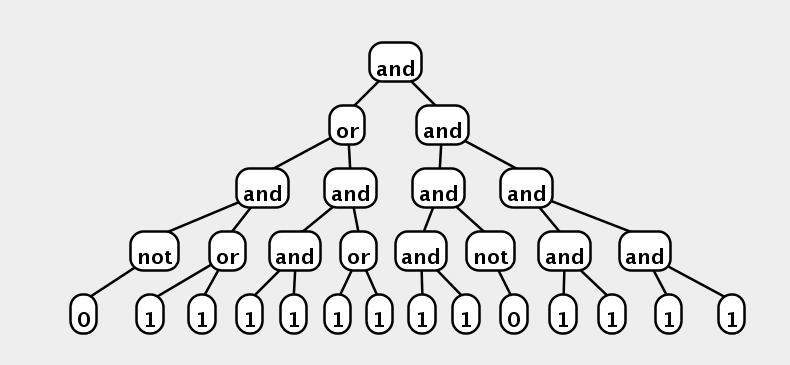
\includegraphics[width=1in]{../board/pics/ss301.png}
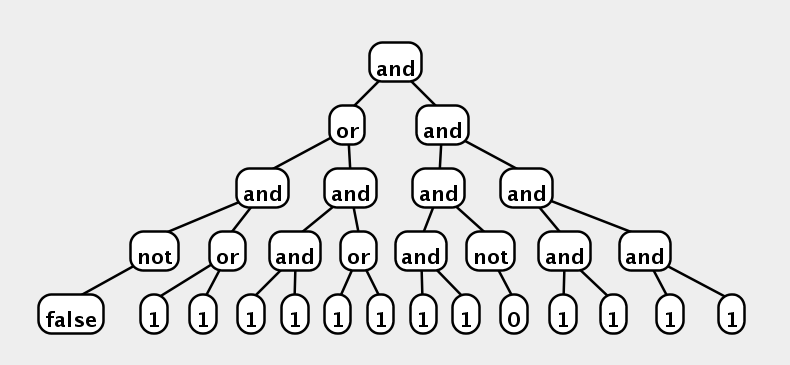
\includegraphics[width=1in]{../board/pics/ss351.png}
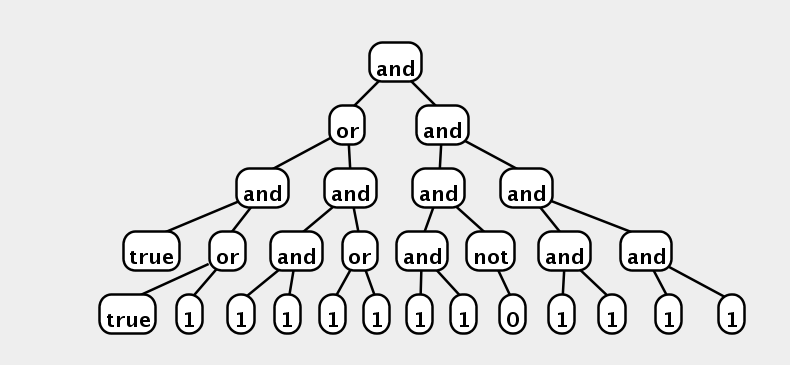
\includegraphics[width=1in]{../board/pics/ss401.png}
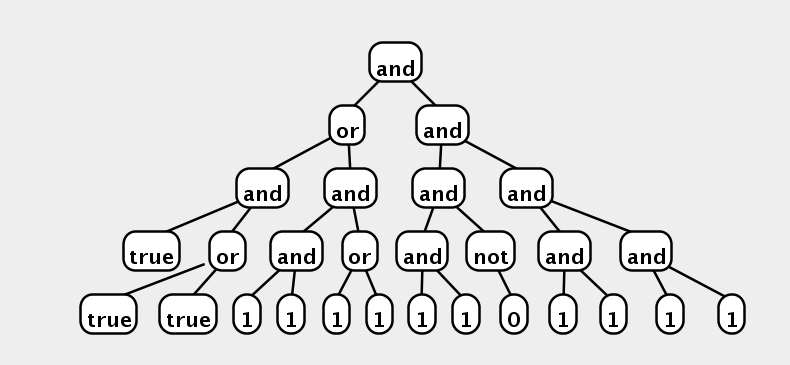
\includegraphics[width=1in]{../board/pics/ss451.png}
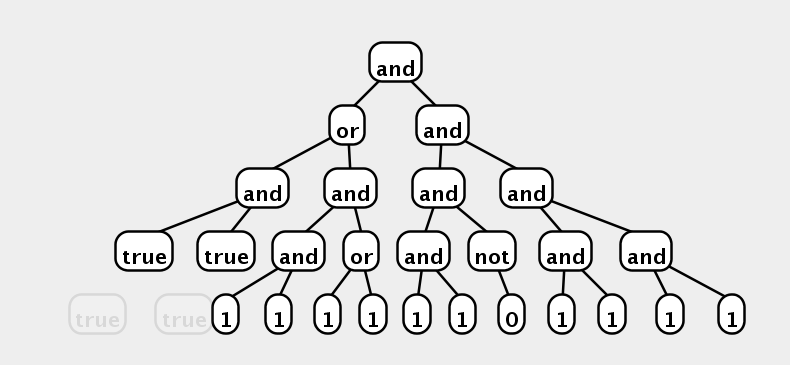
\includegraphics[width=1in]{../board/pics/ss501.png}
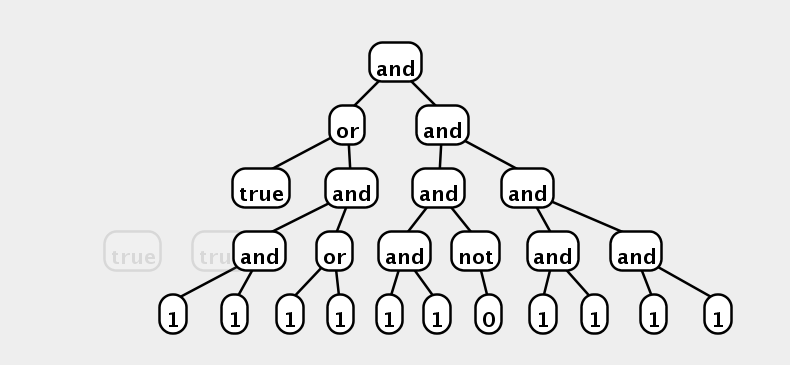
\includegraphics[width=1in]{../board/pics/ss551.png}
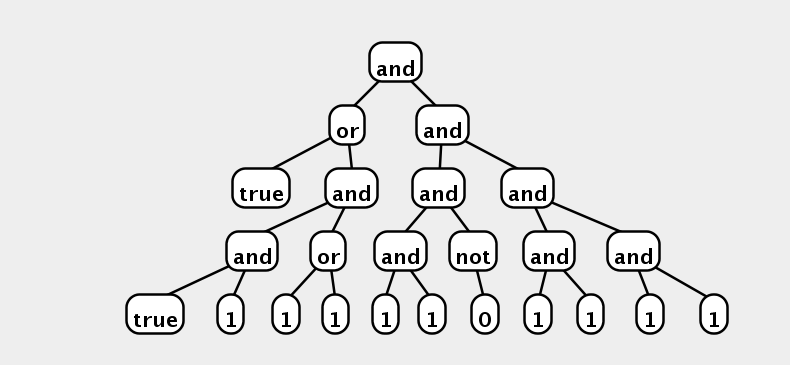
\includegraphics[width=1in]{../board/pics/ss601.png}
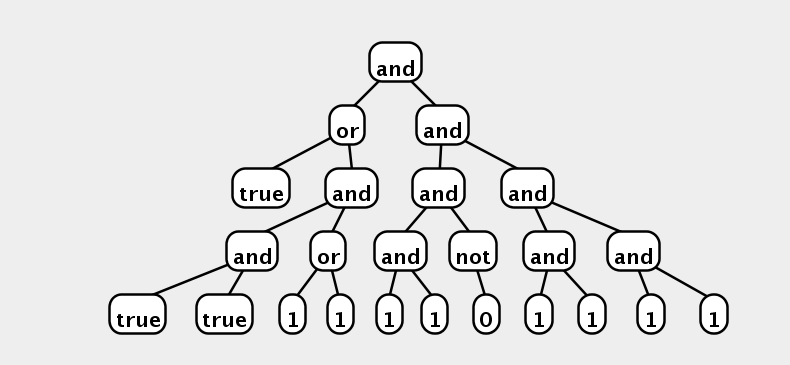
\includegraphics[width=1in]{../board/pics/ss651.png}
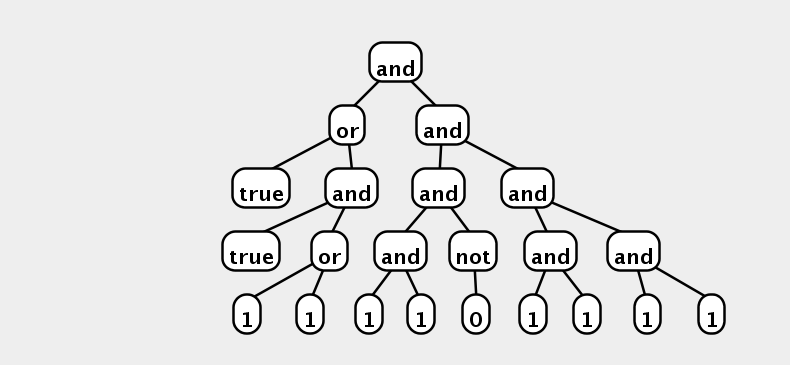
\includegraphics[width=1in]{../board/pics/ss701.png}
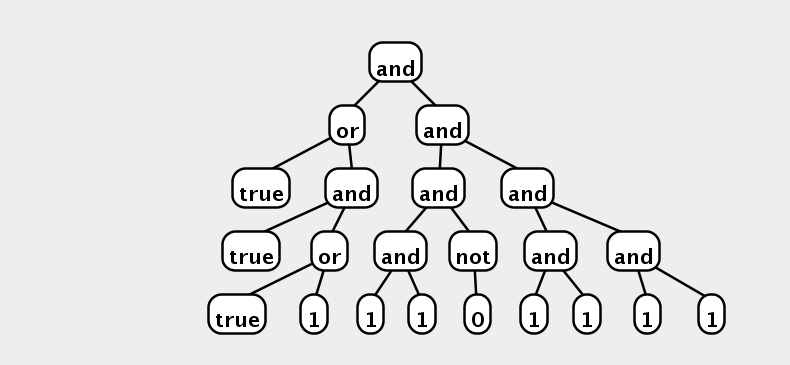
\includegraphics[width=1in]{../board/pics/ss751.png}
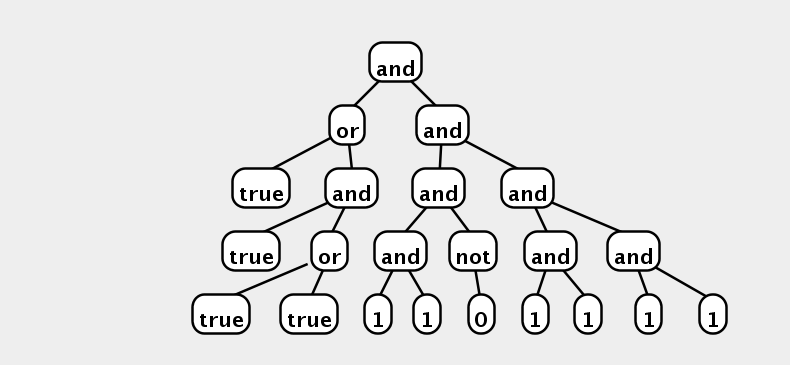
\includegraphics[width=1in]{../board/pics/ss801.png}
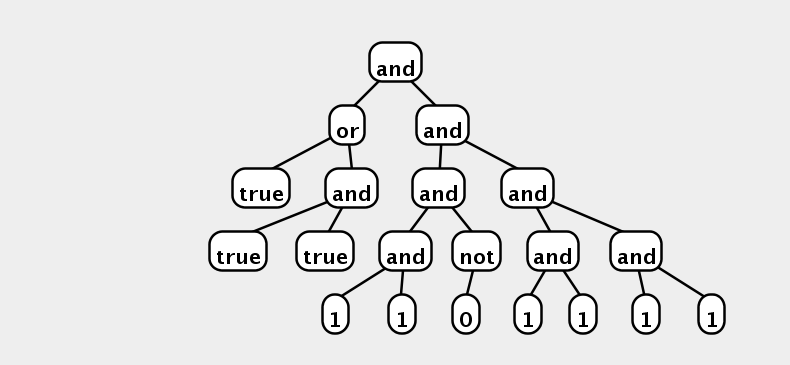
\includegraphics[width=1in]{../board/pics/ss851.png}
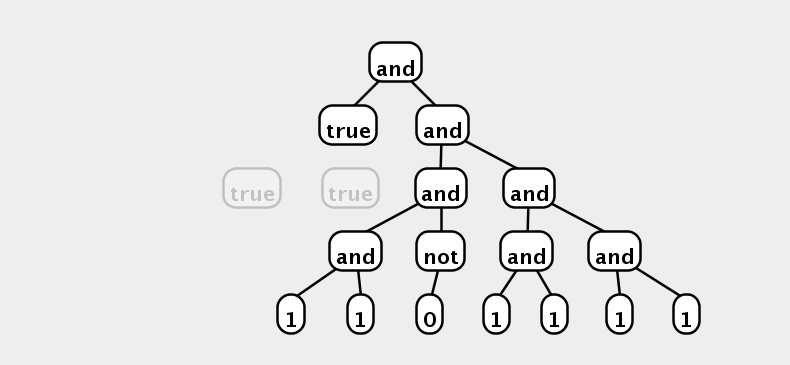
\includegraphics[width=1in]{../board/pics/ss901.png}
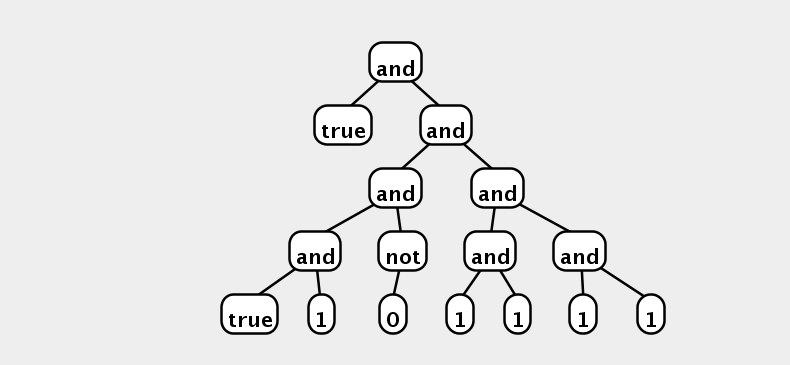
\includegraphics[width=1in]{../board/pics/ss951.png}
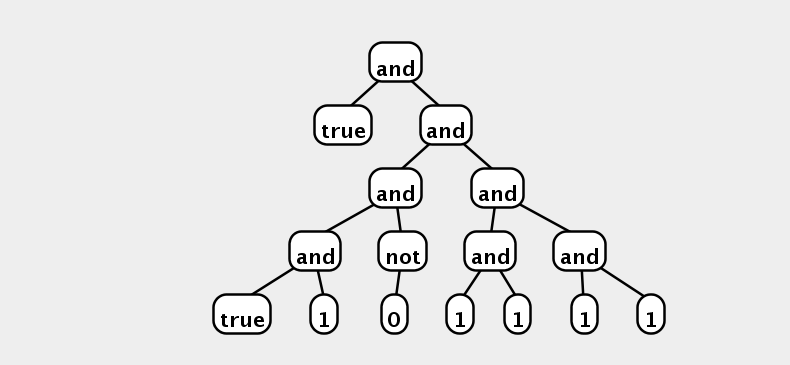
\includegraphics[width=1in]{../board/pics/ss1001.png}
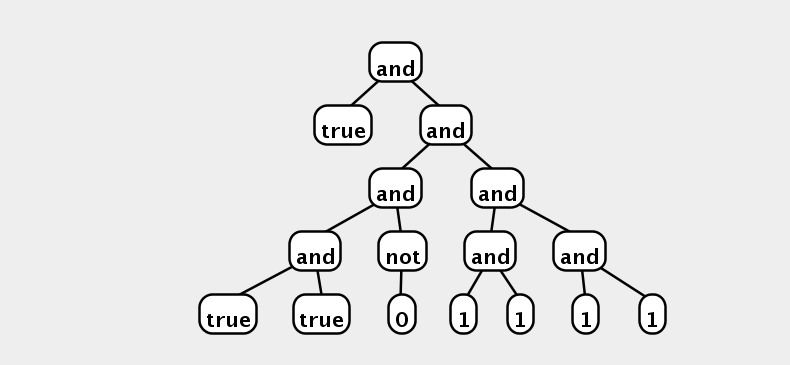
\includegraphics[width=1in]{../board/pics/ss1051.png}
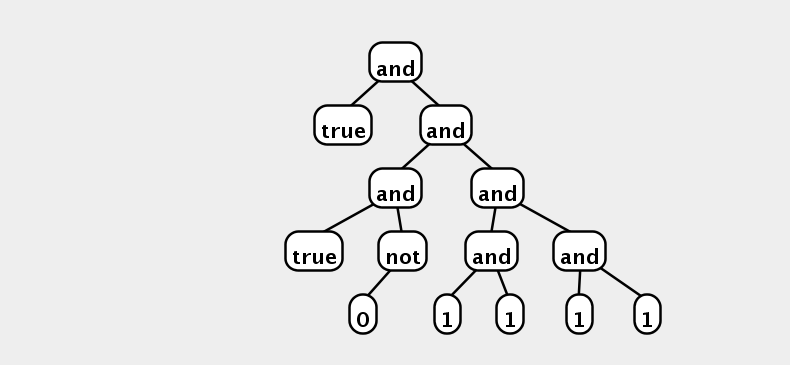
\includegraphics[width=1in]{../board/pics/ss1101.png}
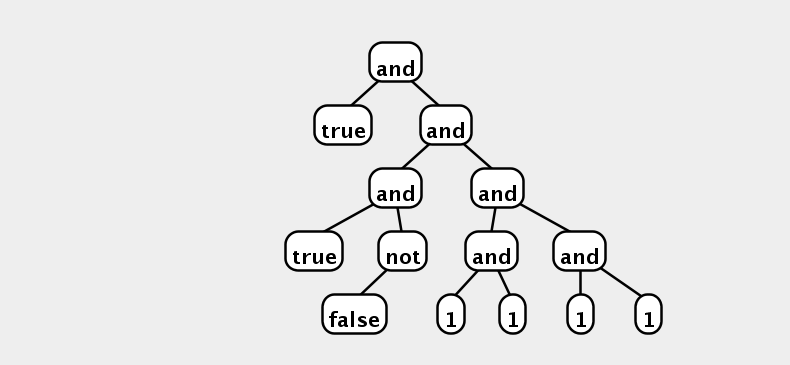
\includegraphics[width=1in]{../board/pics/ss1151.png}
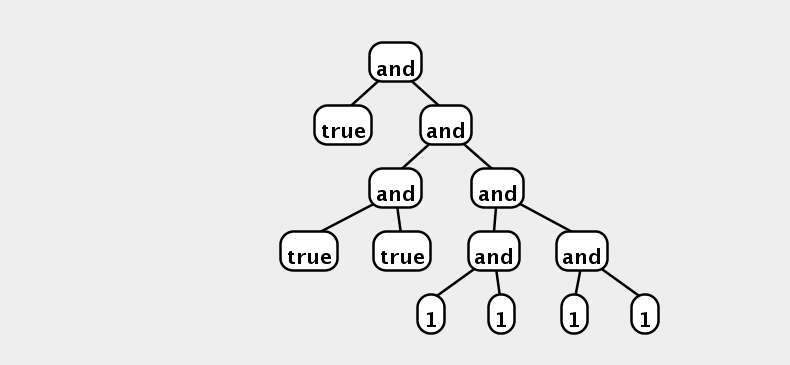
\includegraphics[width=1in]{../board/pics/ss1201.png}
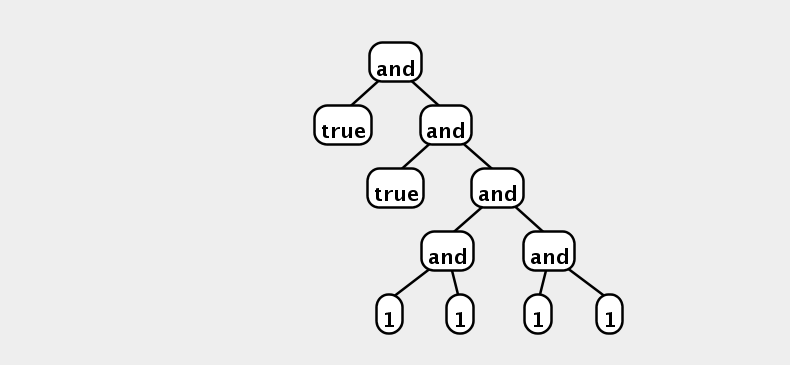
\includegraphics[width=1in]{../board/pics/ss1251.png}
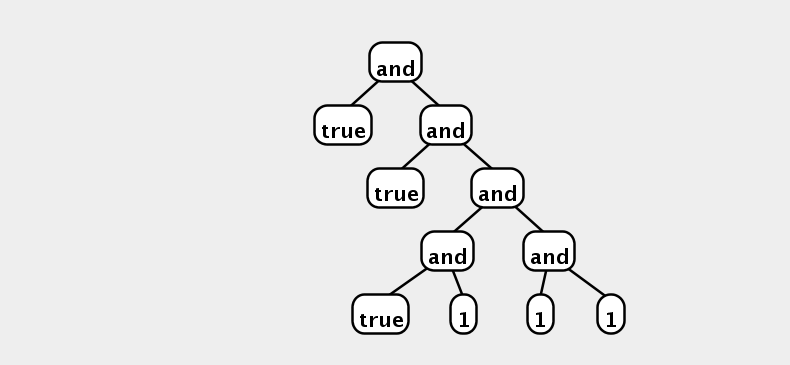
\includegraphics[width=1in]{../board/pics/ss1301.png}
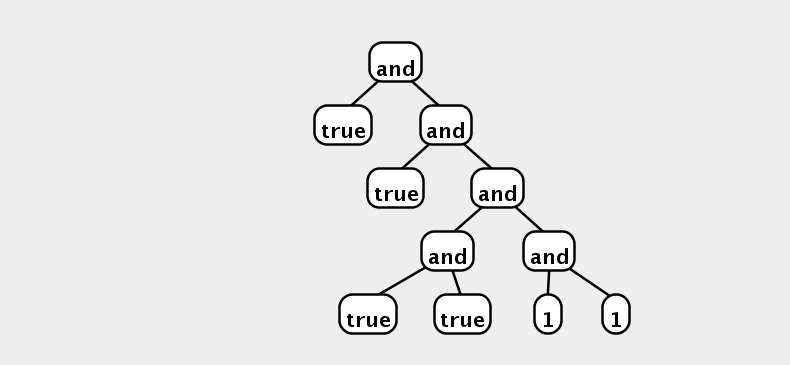
\includegraphics[width=1in]{../board/pics/ss1351.png}
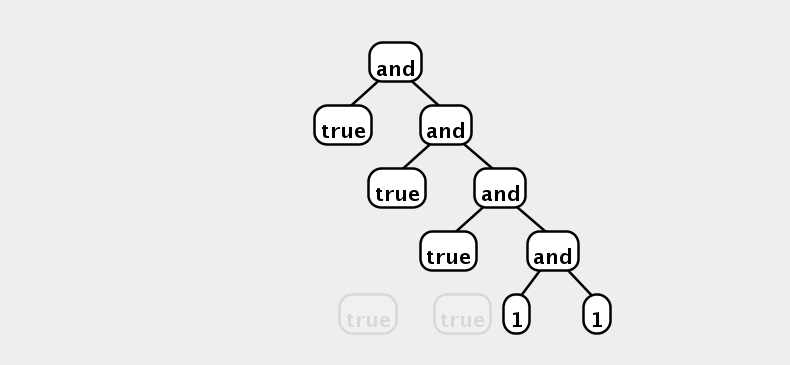
\includegraphics[width=1in]{../board/pics/ss1401.png}
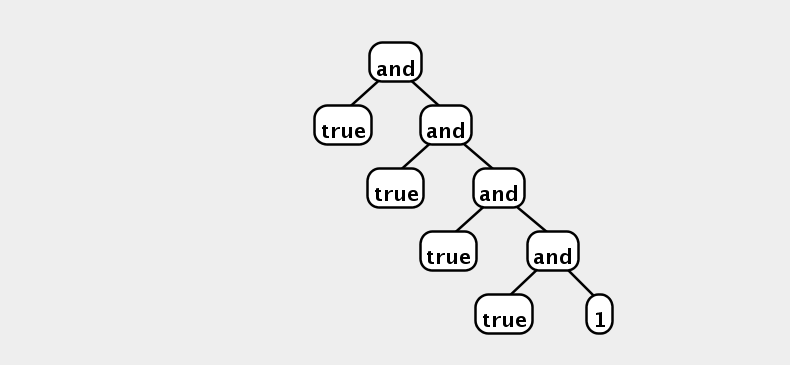
\includegraphics[width=1in]{../board/pics/ss1451.png}
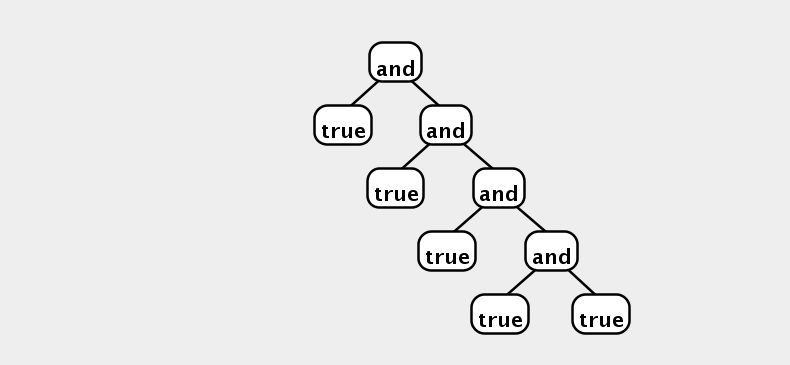
\includegraphics[width=1in]{../board/pics/ss1501.png}
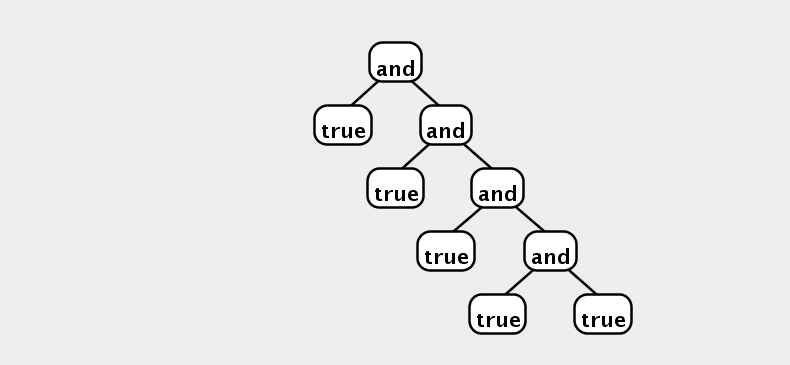
\includegraphics[width=1in]{../board/pics/ss1551.png}
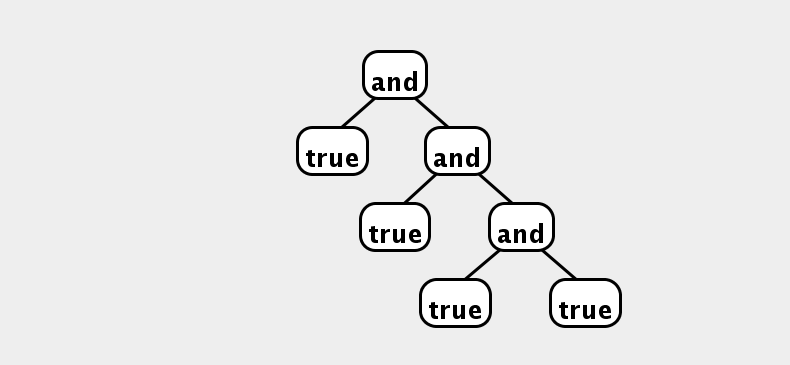
\includegraphics[width=1in]{../board/pics/ss1601.png}
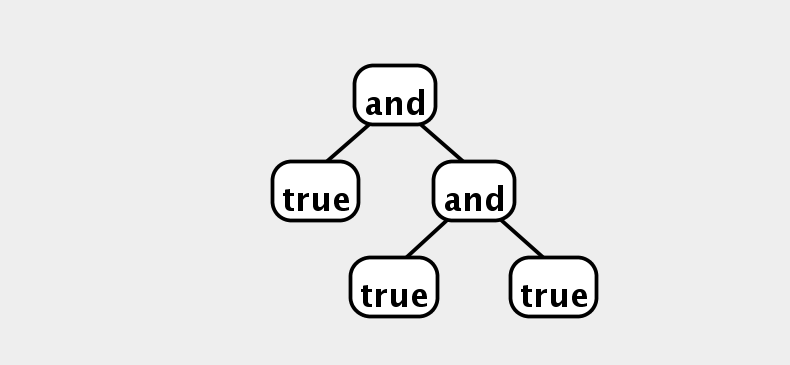
\includegraphics[width=1in]{../board/pics/ss1651.png}
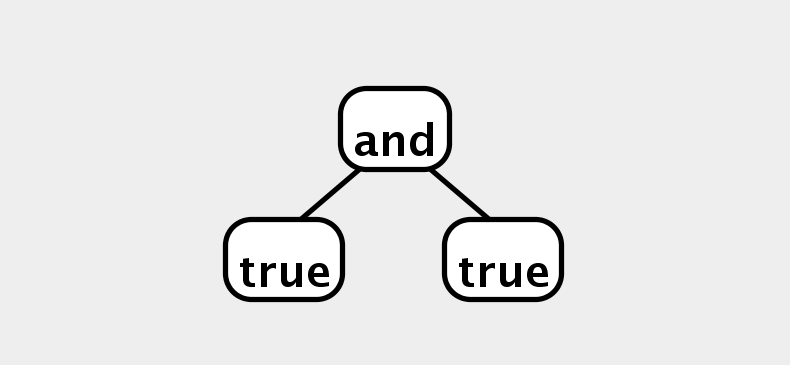
\includegraphics[width=1in]{../board/pics/ss1701.png}

\includegraphics[width=1in]{../board/pics/ss1751.png}

\includegraphics[width=1in]{../board/pics/ss1801.png}
\end{center}
\caption{A flipbook-style visualization of the execution of a tree automaton which recognizes tautologies generated by our library.}
\label{fig:auto}
\end{figure}

Our visualization of a tree automaton was, in our own estimation,
straightforward to create, and it does provide a visualization of the process
of an automaton attempting to recognize a tree.  The animation proceeds in a smooth manner on a laptop purchased in 2008, which indicates that, for a problem of this size, our library is practically useful as well as theoretically fast enough.

\subsection{Example: Lisp}

We also created a visualization of a lisp machine executing a very basic program.  Lisp programs are represented by s-expressions, and these s-expressions directly correspond to a pre-order traversal of a tree.  Thus, we represent the lisp program which calculates one of the roots of $x^2+x-6$ as shown in Figure~\ref{lispprog}.
\begin{figure}
\begin{verbatim}((fun (a b c) 
    (/  (+  (* -1 b) 
            (^ (- (^ b 2) (* 4 (* a c))) .5)) 
        (* 2 a)))  
1 1 -6)
\end{verbatim}
\caption{A Lisp program which calculates one of the roots of $x^2+x-6$ using the quadratic formula.}
\label{lispprog}
\end{figure}

There exist multiple virtual machines which model the execution of lisp code in equivalent manners, here we used one based on string substitution.  The interested reader is referred to {\it Abstract computing Machines} by Kluge\cite{acm}.  This particular visualization took more code than the tree automaton, but it includes the implementation of a Turing-complete lisp compiler and virtual machine, and so may be forgiven for the extra length.  The total length of all the code required was one the order of 450 lines of Java, and so is suitable for a long project or a perhaps a group project in a programming languages course.

The results of our visualization may be found in the animation flipbook shown
in Figure~\ref{lispanim}. In the flipbook, one can see many examples of
vertices caught in the middle of an animation, either fading out or in the process of moving about the screen.  

\begin{figure}
\begin{center}
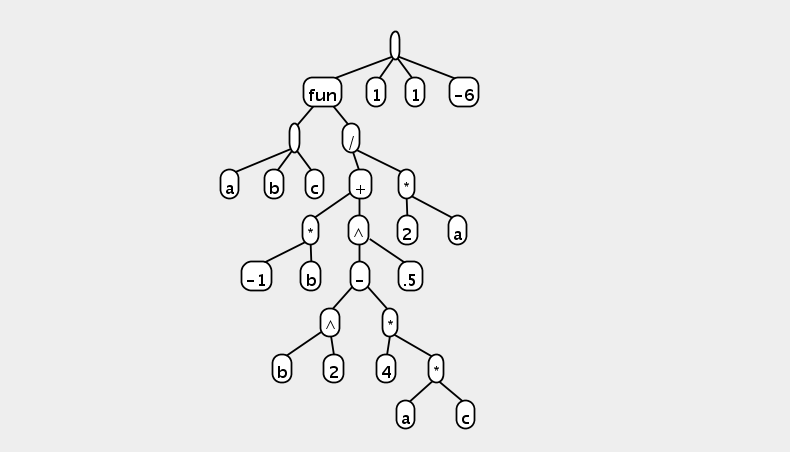
\includegraphics[width=1.25in]{../board/pics/qf1101.png}
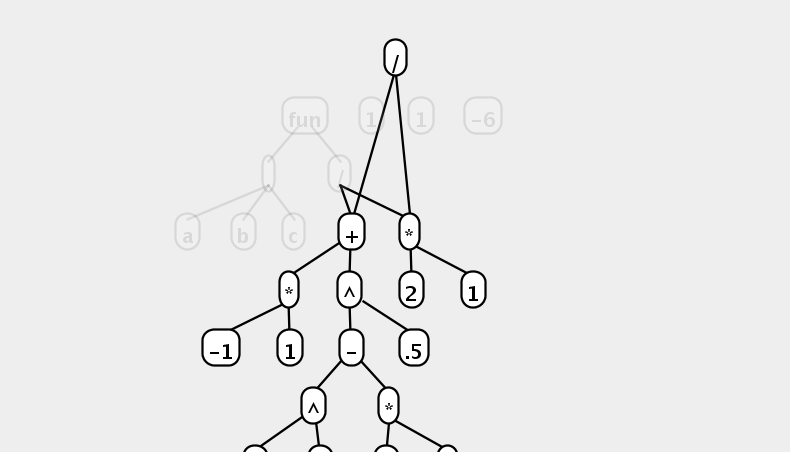
\includegraphics[width=1.25in]{../board/pics/qf1551.png}
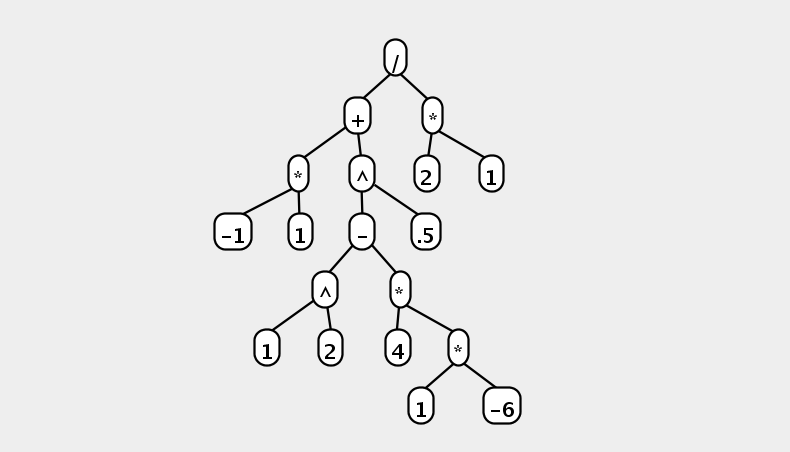
\includegraphics[width=1.25in]{../board/pics/qf1601.png}
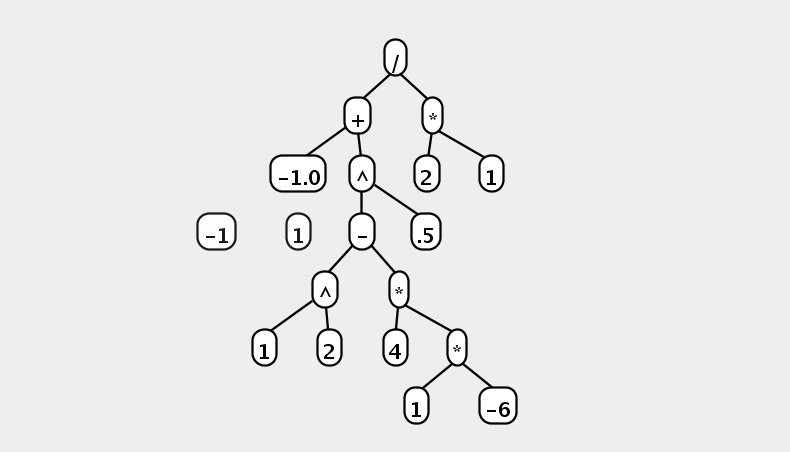
\includegraphics[width=1.25in]{../board/pics/qf1651.png}
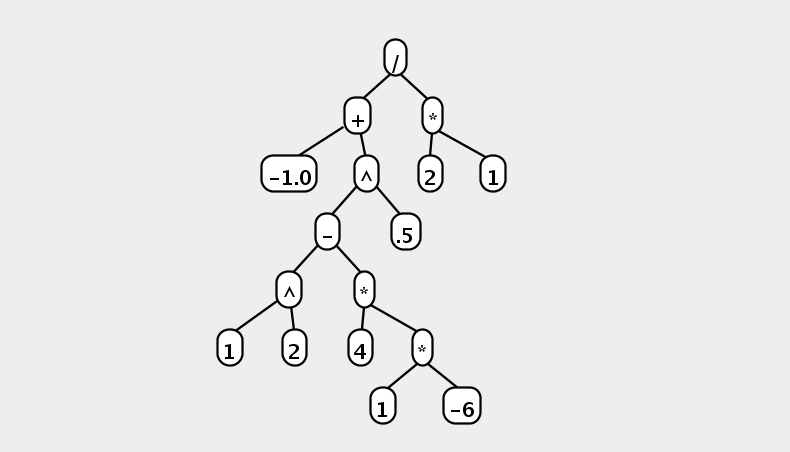
\includegraphics[width=1.25in]{../board/pics/qf1701.png}
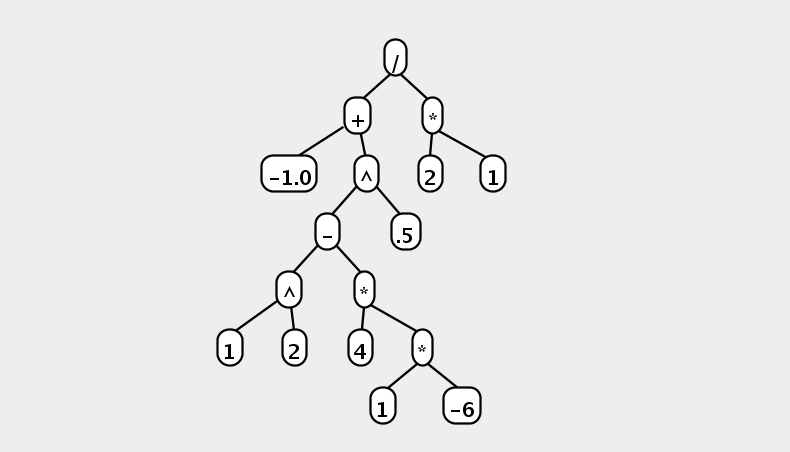
\includegraphics[width=1.25in]{../board/pics/qf1801.png}
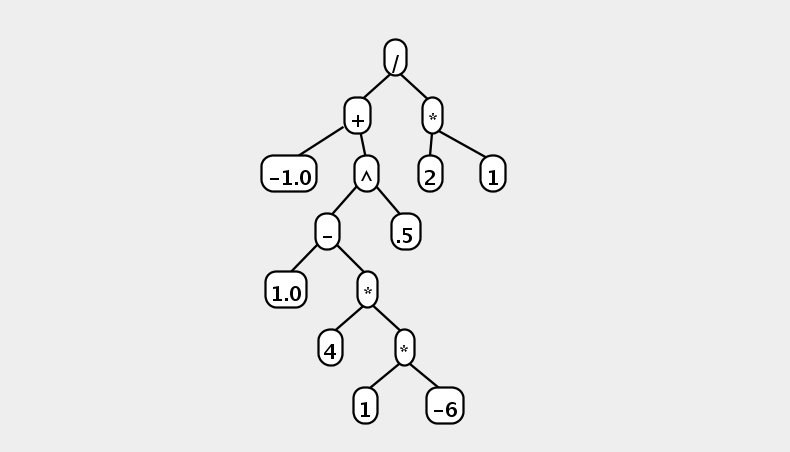
\includegraphics[width=1.25in]{../board/pics/qf1951.png}
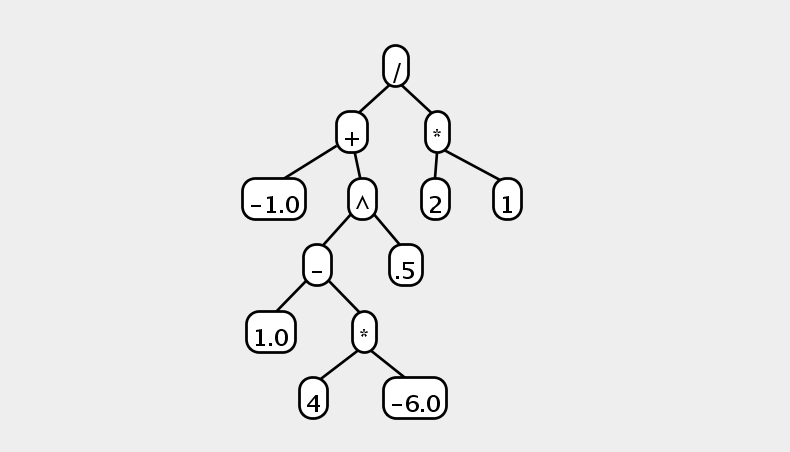
\includegraphics[width=1.25in]{../board/pics/qf2001.png}
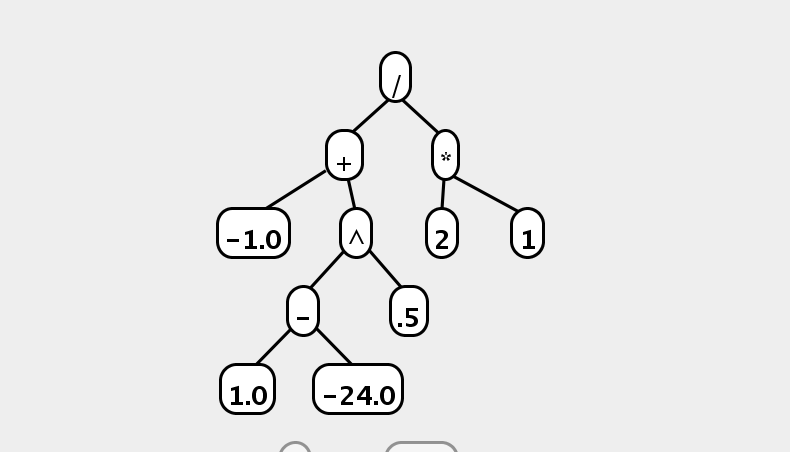
\includegraphics[width=1.25in]{../board/pics/qf2101.png}
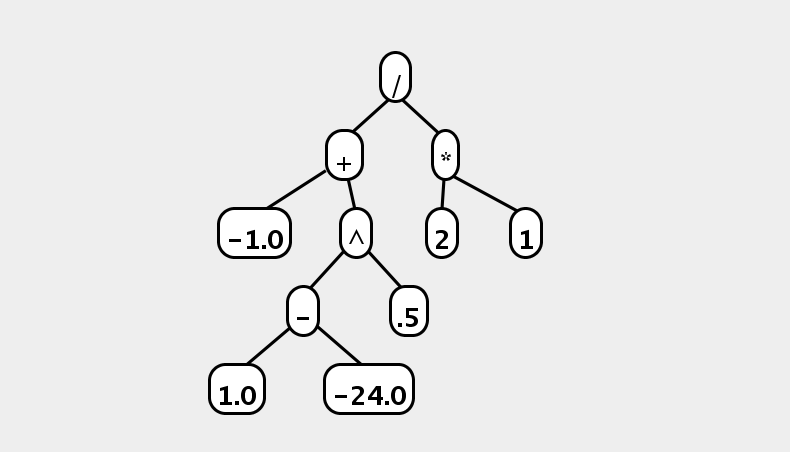
\includegraphics[width=1.25in]{../board/pics/qf2151.png}
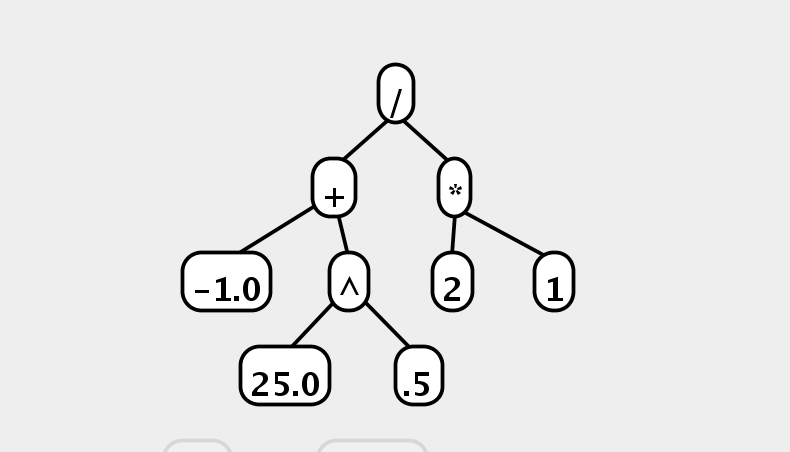
\includegraphics[width=1.25in]{../board/pics/qf2251.png}
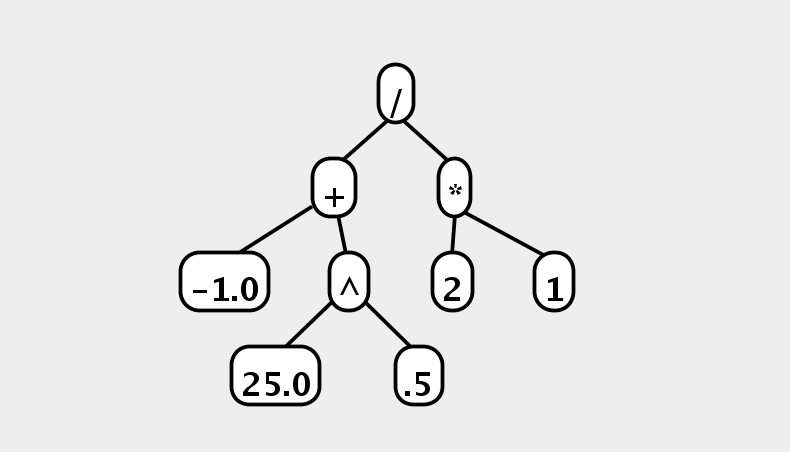
\includegraphics[width=1.25in]{../board/pics/qf2301.png}
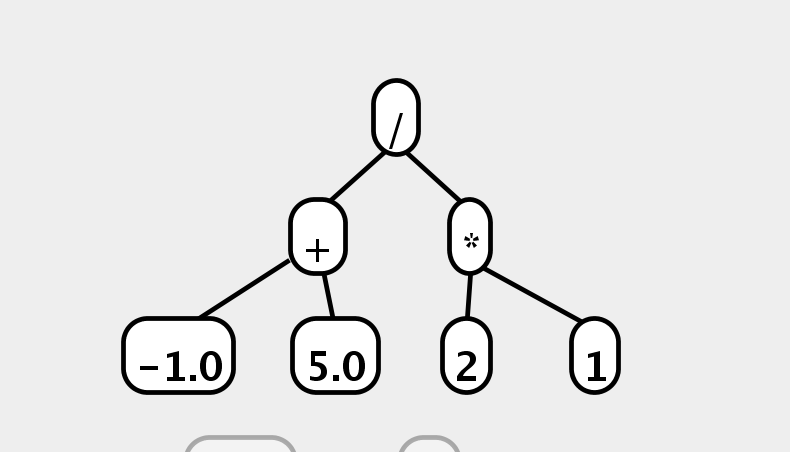
\includegraphics[width=1.25in]{../board/pics/qf2351.png}
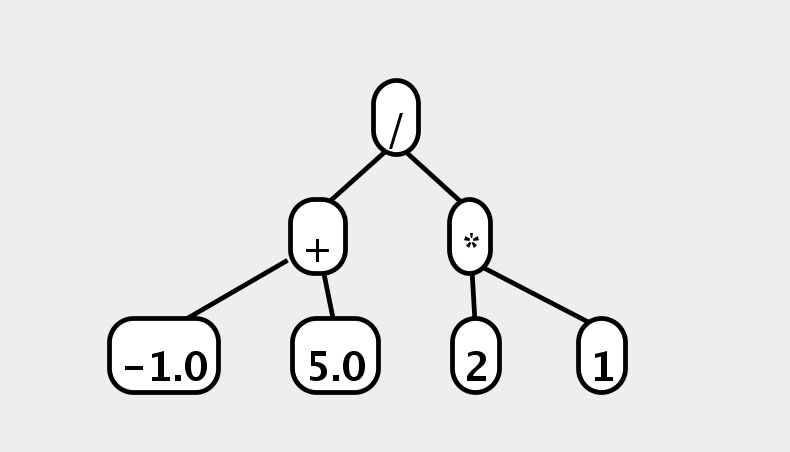
\includegraphics[width=1.25in]{../board/pics/qf2401.png}
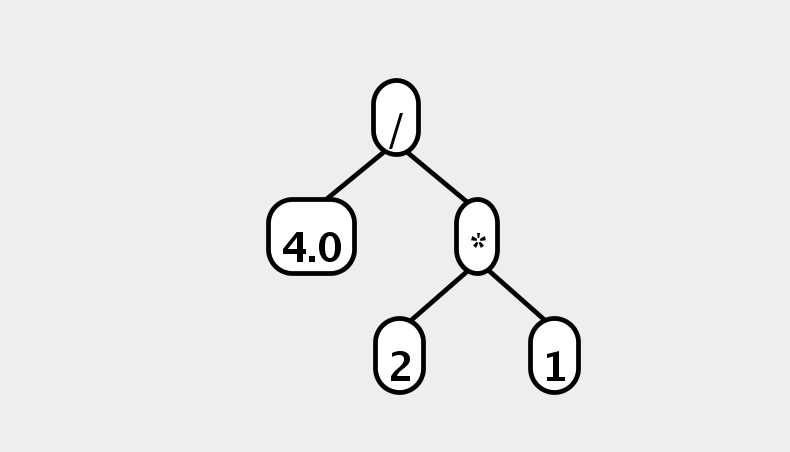
\includegraphics[width=1.25in]{../board/pics/qf2551.png}
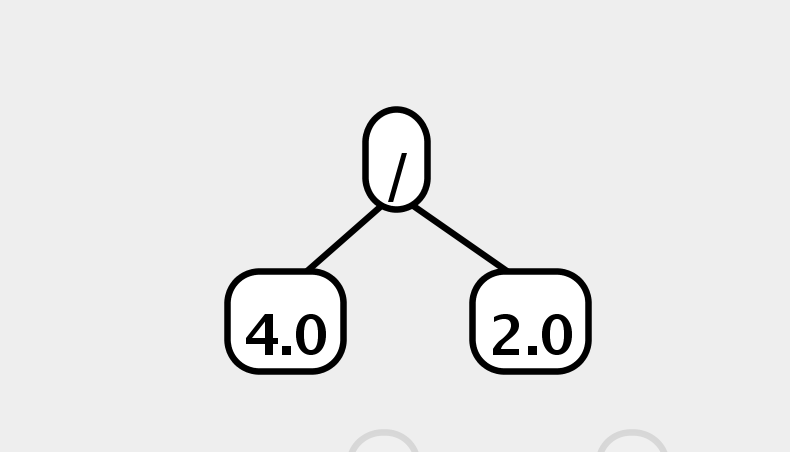
\includegraphics[width=1.25in]{../board/pics/qf2601.png}
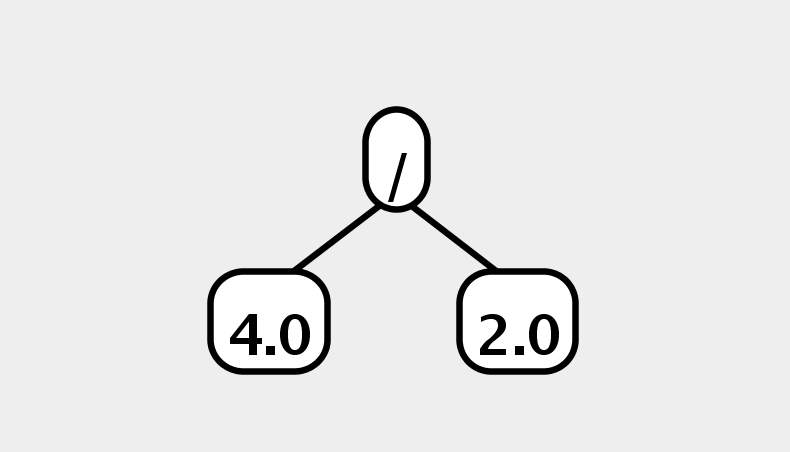
\includegraphics[width=1.25in]{../board/pics/qf2701.png}

\includegraphics[width=1.25in]{../board/pics/qf2801.png}
\end{center}
\caption{The complete execution of a lisp program calculating one of the roots of $x^2+x-6$.}
\label{lispanim}
\end{figure}

As well as the execution of the evaluation of the quadratic formula, we have
also produced visualizations of lisp code calculating the factorial function
and the Fibonacci sequence.  These examples, while interesting, are mostly
interesting as examples of the $\lambda$-calculus and teaching aids in a
programming languages course.  The animation proceeds much like the flipbook
shown, but the trees involved are much larger and more intricate.

\subsection{Other Example Visualizations}

Also included with our library are visualizations of self-adjusting binary
search trees (AVL Trees) and of the growth of a random tree.  The random tree
is particularly interesting, because it was requested by an audience member
during a presentation and was then implemented in the next half hour.  We hope
that this short distance from request to implementation can serve as an example
of the power of both our library and especially our design approach.

\section{Conclusion}

We have passed a threshold of computational abundance which can allow
visualization libraries to use less-efficient algorithms in pursuit of
programming ease.  Noting this threshold allows us to articulate a design for a
layout library that, by doing much more work behind the scenes, makes the
creation of visualizations available to a much larger audience.  We have
created such a library and provided several sample visualizations.  We hope
that any and all of our design ideas, the resulting library\cite{ourlibrary},
and the provided visualizations, might be useful to others who are attempting
to demonstrate, learn, understand, or admire the behavior of trees which evolve
over time.

\bibliographystyle{abbrv}
\bibliography{bibliography.bib}

\end{document}
